\documentclass{article}
\usepackage{arxiv}

\usepackage[utf8]{inputenc}
\usepackage[english, russian]{babel}
\usepackage[T1]{fontenc}
\usepackage{url}
\usepackage{booktabs}
\usepackage{amsfonts}
\usepackage{nicefrac}
\usepackage{microtype}
\usepackage{lipsum}
\usepackage{graphicx}
\usepackage{natbib}
\usepackage{doi}



\title{Mitigating distributional biases in contrastive learning}

\author{ Lidia Troeshestova \\
	Moscow Institute of Physics and Technology\\
	\texttt{troeshestova.ls@phystech.edu} \\
	%% examples of more authors
	\And
	Roman Isachenko\thanks{Use footnote for providing further information about author (webpage, alternative address)---\emph{not} for acknowledging funding agencies.} \\
	   \\
	\texttt{} \\
	%% \AND
	%% Coauthor \\
	%% Affiliation \\
	%% Address \\
	%% \texttt{email} \\
	%% \And
	%% Coauthor \\
	%% Affiliation \\
	%% Address \\
	%% \texttt{email} \\
	%% \And
	%% Coauthor \\
	%% Affiliation \\
	%% Address \\
	%% \texttt{email} \\
}
\date{}

\renewcommand{\shorttitle}{\textit{arXiv} Template}

%%% Add PDF metadata to help others organize their library
%%% Once the PDF is generated, you can check the metadata with
%%% $ pdfinfo template.pdf
\hypersetup{
pdftitle={A template for the arxiv style},
pdfsubject={q-bio.NC, q-bio.QM},
pdfauthor={David S.~Hippocampus, Elias D.~Striatum},
pdfkeywords={First keyword, Second keyword, More},
}

\begin{document}
\maketitle

\begin{abstract}
	Recently there has been a renewed interest in using contrastive learning for self-supervised representation learning. A popular method for learning representations without labels is to compare similar (positive) and dissimilar (negative) pairs of samples. However, negative samples are often chosen randomly, which means that they could be of the same class. This paper analyzes various ways to eliminate these biases. Based on the fully-supervised case, we develop debiased contrastive models that account for same-label datapoints without requiring knowledge of true labels, and explore their properties. The experiments are performed on MNIST and CIFAR10 datasets. This can further improve availability of accurate models for classification in tasks where extensive labeling is expensive or inaccessible.
\end{abstract}


\keywords{: Contrastive learning \and Representation learning \and Self-supervised learning}

\section{Introduction}
Representation learning has become increasingly popular in recent years due to its ability to learn meaningful representations from large amounts of data, without the need for manual feature engineering. A widely used solution for this problem is contrastive learning, a technique that uses the principle of contrasting samples against each other to learn attributes that are common between data classes and attributes that set apart a data class from another. It encourages the representations of similar pairs $(x, x^+)$ to be close, and those of dissimilar pairs $(x, x^-)$ to be more orthogonal.

Due to the unavailability of actual labels during training, negative instances $x^-$ are often randomly selected from the training data. However, this approach can result in sampling bias, where $x^-$ may actually be similar to $x$. This bias can cause a significant drop in performance. 

To address this issue, \citep{khosla2021supervised} extend the self-supervised batch contrastive approach to the fully-supervised setting, allowing to effectively leverage label information. According to the experiments, supervised contrastive loss outperforms the base cross entropy, but only by a small amount. It also outperforms the cross entropy on robustness benchmark (ImageNet-C, which applies common naturally occuring perturbations such as noise, blur and contrast changes to the ImageNet dataset) and is less sensitive to hyperparameter changes.

\citep{chuang2021debiased} proposed an unbiased method, where $x$ is drawn from data with labels that are truly different from $x$.

\citep{chuang2021debiased} introduced \emph{debiased contrastive loss}.



\section{Problem Statement}
\label{sec:headings}

\lipsum[4] See Section \ref{sec:headings}.

\subsection{Headings: second level}
\lipsum[5]
\begin{equation}
	\xi _{ij}(t)=P(x_{t}=i,x_{t+1}=j|y,v,w;\theta)= {\frac {\alpha _{i}(t)a^{w_t}_{ij}\beta _{j}(t+1)b^{v_{t+1}}_{j}(y_{t+1})}{\sum _{i=1}^{N} \sum _{j=1}^{N} \alpha _{i}(t)a^{w_t}_{ij}\beta _{j}(t+1)b^{v_{t+1}}_{j}(y_{t+1})}}
\end{equation}

\subsubsection{Headings: third level}
\lipsum[6]

\paragraph{Paragraph}
\lipsum[7]



\section{Examples of citations, figures, tables, references}
\label{sec:others}

\subsection{Citations}
Citations use \verb+natbib+. The documentation may be found at
\begin{center}
	\url{http://mirrors.ctan.org/macros/latex/contrib/natbib/natnotes.pdf}
\end{center}

Here is an example usage of the two main commands (\verb+citet+ and \verb+citep+): Some people thought a thing \citep{kour2014real, hadash2018estimate} but other people thought something else \citep{kour2014fast}. Many people have speculated that if we knew exactly why \citet{kour2014fast} thought this\dots

\subsection{Figures}
\lipsum[10]
See Figure \ref{fig:fig1}. Here is how you add footnotes. \footnote{Sample of the first footnote.}
\lipsum[11]

\begin{figure}
	\centering
	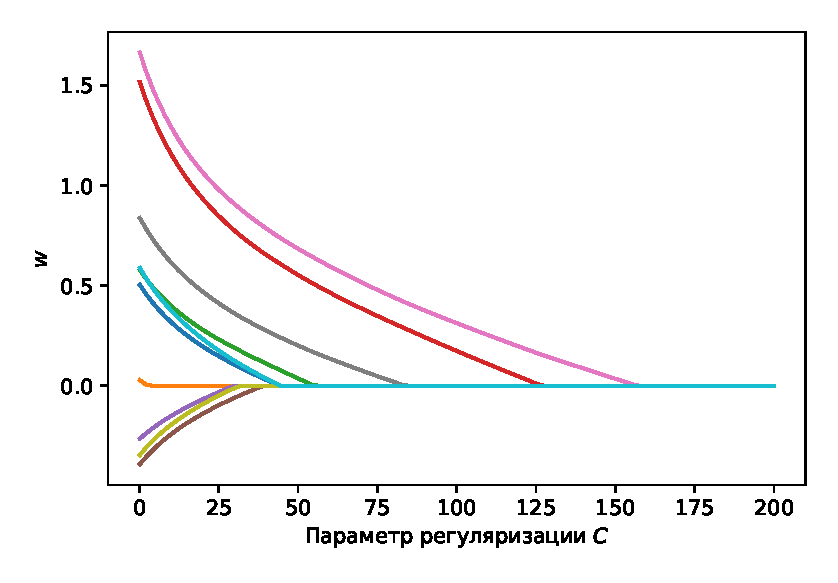
\includegraphics[width=0.5\textwidth]{../figures/log_reg_cs_exp.eps}
	\caption{Sample figure caption.}
	\label{fig:fig1}
\end{figure}

\subsection{Tables}
See awesome Table~\ref{tab:table}.

The documentation for \verb+booktabs+ (`Publication quality tables in LaTeX') is available from:
\begin{center}
	\url{https://www.ctan.org/pkg/booktabs}
\end{center}


\begin{table}
	\caption{Sample table title}
	\centering
	\begin{tabular}{lll}
		\toprule
		\multicolumn{2}{c}{Part}                   \\
		\cmidrule(r){1-2}
		Name     & Description     & Size ($\mu$m) \\
		\midrule
		Dendrite & Input terminal  & $\sim$100     \\
		Axon     & Output terminal & $\sim$10      \\
		Soma     & Cell body       & up to $10^6$  \\
		\bottomrule
	\end{tabular}
	\label{tab:table}
\end{table}

\subsection{Lists}
\begin{itemize}
	\item Lorem ipsum dolor sit amet
	\item consectetur adipiscing elit.
	\item Aliquam dignissim blandit est, in dictum tortor gravida eget. In ac rutrum magna.
\end{itemize}


\bibliographystyle{unsrtnat}
\bibliography{references}

\end{document}